\documentclass[a4paper,1pt]{report}
\usepackage[utf8]{inputenc}
\usepackage{amsfonts}
\usepackage{amsthm}
\usepackage{amssymb}
\usepackage{amsmath}
\usepackage{graphicx}
\usepackage{subcaption}
\usepackage{float}

\newtheorem*{pbo}{Principio del Buen Ordenamiento}

\newtheorem*{pim}{Principio de Inducción Matemática}

\newtheorem*{teo}{Teorema}

\newtheorem*{cor}{Corolario}

\newtheorem*{dem}{Demostración}

\newtheorem*{dfn}{Definición}

\newtheorem*{lem}{Lema}

\newtheorem*{prp}{Propiedades}


% Title Page
\title{Conferencia 2 - \'Arboles y Secuencia Gr\'afica}
\author{}



\begin{document}
\maketitle

%\begin{abstract}
%\end{abstract}

\begin{dfn}[$P_n$]
    Se denomina $P_n$ al grafo con $n$ v\'ertices $V(G)= \{v_1, v_2,..., v_n\}$ y con aristas $E(G) = \{\{v_1, v_2\},\{v_2, v_3\}, \{v_3, v_4\},...,\{v_{n-1}, v_{n}\} \}$ 
\end{dfn}

\begin{figure}[H]
    \centering
    \begin{subfigure}[b]{0.30\textwidth}
    \centering
    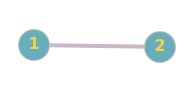
\includegraphics[width=0.5\textwidth]{figures2/P2.png}
    \caption{$P_2$}
    \end{subfigure}
    \begin{subfigure}[b]{0.30\textwidth}
        \centering
    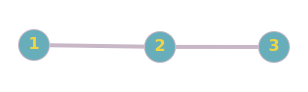
\includegraphics[width=0.75\textwidth]{figures2/P3.png}
    \caption{$P_3$}
    \end{subfigure}
    \begin{subfigure}[b]{0.30\textwidth}
        \centering
    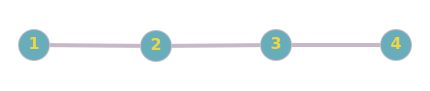
\includegraphics[width=0.95\textwidth]{figures2/P4.png}
    \caption{$P_4$}
    \end{subfigure}
\end{figure} 

\begin{dfn}[$C_n$]
    Se denomina $C_n$ ($n \geq 3$) al grafo c\'iclico con $n$ v\'ertices $V(G)= \{v_1, v_2,..., v_n\}$  y con aristas $E(G) = \{\{v_1, v_2\},\{v_2, v_3\},...,\{v_{n-1}, v_{n}\}, \{v_{n}, v_{1}\}\}$ 
\end{dfn}

\begin{figure}[H]
    \centering
    \begin{subfigure}[b]{0.30\textwidth}
    \centering
    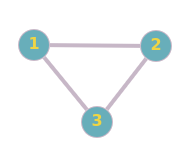
\includegraphics[width=0.5\textwidth]{figures2/C3.png}
    \caption{$C_3$}
    \end{subfigure}
    \begin{subfigure}[b]{0.30\textwidth}
        \centering
    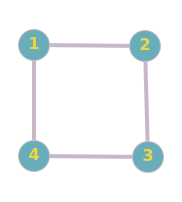
\includegraphics[width=0.5\textwidth]{figures2/C4.png}
    \caption{$C_4$}
    \end{subfigure}
    \begin{subfigure}[b]{0.30\textwidth}
        \centering
    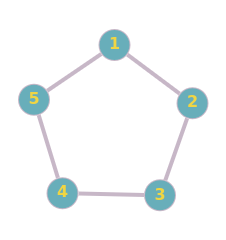
\includegraphics[width=0.5\textwidth]{figures2/C5.png}
    \caption{$C_5$}
    \end{subfigure}
\end{figure} 

\begin{dfn}[$K_n$]
    Se denomina $K_n$ al grafo completo con $n$ v\'ertices $V(G)= \{v_1, v_2,..., v_n\}$  donde $\forall v_i, v_j \in V(G), i\neq j$ la arista $\{v_i, v_j\} \in E(G)$, es decir es el grafo con $\binom{n}{2}$ aristas.
\end{dfn}

\begin{figure}[H]
    \centering
    \begin{subfigure}[b]{0.22\textwidth}
    \centering
    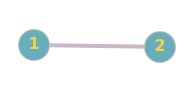
\includegraphics[width=0.5\textwidth]{figures2/P2.png}
    \caption{$K_2$}
    \end{subfigure}
    \begin{subfigure}[b]{0.22\textwidth}
        \centering
    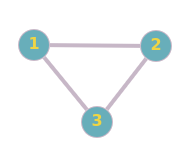
\includegraphics[width=0.5\textwidth]{figures2/C3.png}
    \caption{$K_3$}
    \end{subfigure}
    \begin{subfigure}[b]{0.22\textwidth}
        \centering
    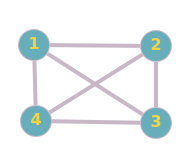
\includegraphics[width=0.5\textwidth]{figures2/K4.png}
    \caption{$K_4$}
    \end{subfigure}
    \begin{subfigure}[b]{0.22\textwidth}
        \centering
    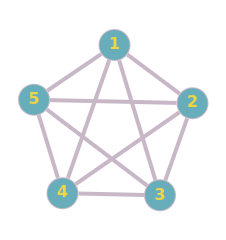
\includegraphics[width=0.5\textwidth]{figures2/K5.png}
    \caption{$K_5$}
    \end{subfigure}
\end{figure} 

\begin{dfn}[Grafo de Petersen]
    Es el grafo de $10$ v\'ertices, regular de grado $3$ cuyos vértices adyacentes
    no tienen vértices comunes y los vértices no adyacentes tienen exactamente un vértice común.
\end{dfn}

\begin{figure}[H]
    \centering
    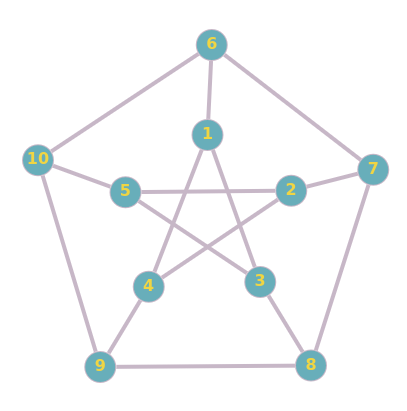
\includegraphics[width=0.2\textwidth]{figures2/Petersen.png}
    \caption{Grafo de Petersen}
\end{figure}

\begin{dfn}[Grafo Complemento]
    Se define como grafo complemento de $G$, al grafo $G^c$, tal que $V(G) = V(G^c)$ y $E(G^c) = [V(G)]^2 / E(G)$, es decir es el grafo que tiene los mismos v\'ertices que $G$, pero que tiene las aristas que no est\'an en $G$.
\end{dfn}

\begin{cor}
  Sea $|V(G)| = n$,  $G \cup G^c = K_n$
\end{cor}


\begin{figure}[H]
    \centering
    \begin{subfigure}[b]{0.30\textwidth}
    \centering
    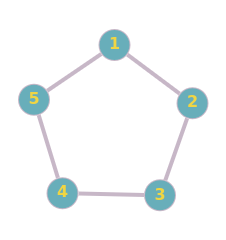
\includegraphics[width=0.5\textwidth]{figures2/C5.png}
    \caption{$G$}
    \end{subfigure}
    \begin{subfigure}[b]{0.30\textwidth}
        \centering
    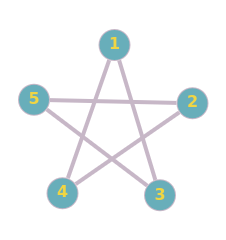
\includegraphics[width=0.5\textwidth]{figures2/C5comp.png}
    \caption{$G^c$}
    \end{subfigure}
    \begin{subfigure}[b]{0.30\textwidth}
        \centering
    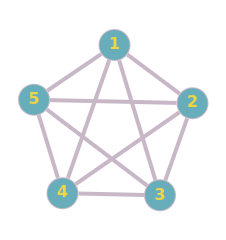
\includegraphics[width=0.5\textwidth]{figures2/K5.png}
    \caption{$G \cup G^c = K_5$}
    \end{subfigure}
    \caption{Ejemplo de grafo y su complemento}
\end{figure} 

\begin{dfn}[Grafo conexo]
    Un grafo es conexo si para todo par de vértices existe un camino que los conecta.
\end{dfn}

\begin{dfn}[Componente Conexa]
    Subgrafo maximal conexo de un grafo
\end{dfn}

\textbf{Nota:} Si un grafo no es conexo entonces tiene 2 o m\'as componentes conexas.

\begin{dfn}
    Un v\'ertice o una arista se denomina de corte si su eliminaci\'on aumenta la cantidad de componentes conexas. A las aristas de corte tambi\'en se les denomina \textbf{Arista puente} y a los v\'ertices de corte \textbf{punto de articulaci\'on}. 
\end{dfn}

\begin{figure}[H]
    \centering
    \begin{subfigure}[b]{0.45\textwidth}
    \centering
    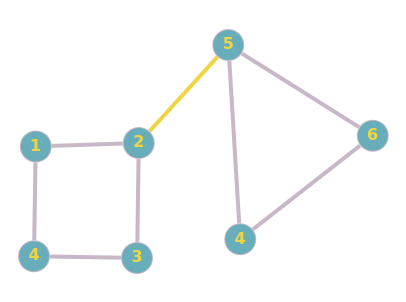
\includegraphics[width=0.5\textwidth]{figures2/aristaCorte.png}
    \caption{La arista $\{2,5\}$ es de corte.}
    \end{subfigure}
    \begin{subfigure}[b]{0.45\textwidth}
        \centering
    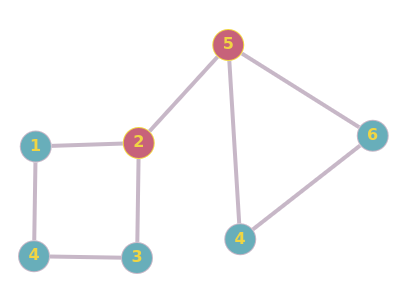
\includegraphics[width=0.5\textwidth]{figures2/verticesCorte.png}
    \caption{Los v\'ertices $2$ y $5$ son de corte}
    \end{subfigure}
\end{figure} 

\begin{figure}[H]
    \centering
    \begin{subfigure}[b]{0.45\textwidth}
    \centering
    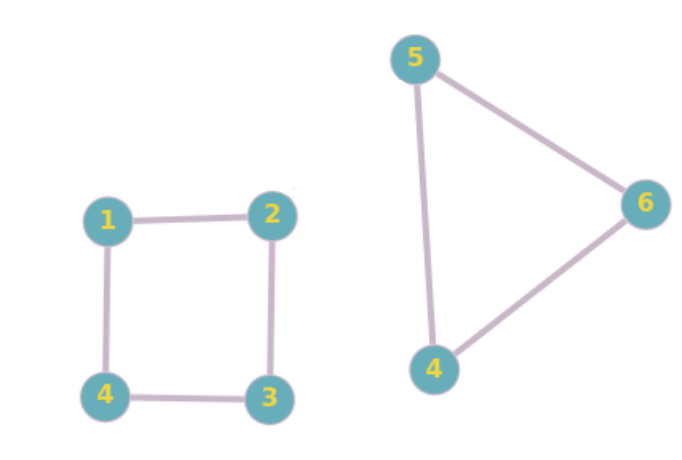
\includegraphics[width=0.26\textwidth]{figures2/G-E.png}
    \caption{$G - \{2,5\}$}
    \end{subfigure}
    \begin{subfigure}[b]{0.22\textwidth}
        \centering
    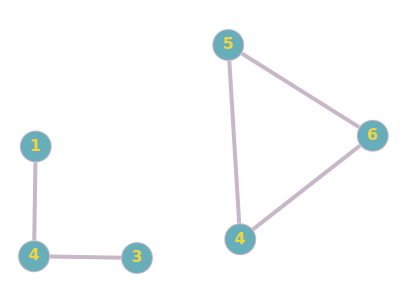
\includegraphics[width=0.5\textwidth]{figures2/G-2.png}
    \caption{$G - 2$}
    \end{subfigure}
    \begin{subfigure}[b]{0.22\textwidth}
    \centering
    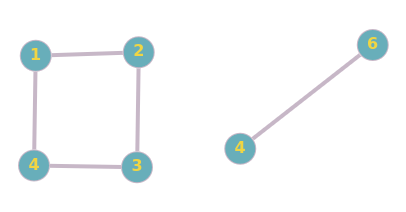
\includegraphics[width=0.5\textwidth]{figures2/G-5.png}
    \caption{$G - 5$}
    \end{subfigure}
    \caption{Al quitar una arista o un v\'ertice de corte el grafo se desconecta}
\end{figure} 

\begin{dfn}[Grafo k-conexo]
    Un grafo $G$ es k-conexo si es $(k-1)$-conexo y para todo $A \subseteq V(G)$ tal que $|A| =k-1$ el grafo $G'= G -A$ es conexo.
\end{dfn}

\textbf{Nota:} Un grafo $2$-conexo (biconexo) es un grafo conexo que no tiene v\'ertices de corte.

\begin{dfn}[Bosque]
    Grafo que no tiene ciclos (ac\'iclico).
\end{dfn}

\begin{figure}[H]
    \centering
    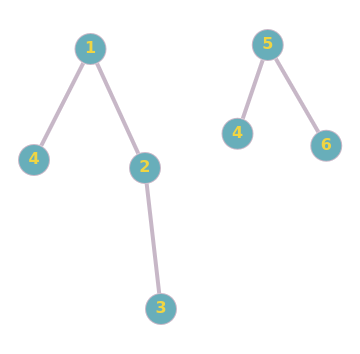
\includegraphics[width=0.2\textwidth]{figures2/bosque.png}
    \caption{Ejemplo de bosque}
\end{figure}


\begin{teo}
    Si $G$ es un bosque con al menos una arista, entonces en $G$ hay al menos dos v\'ertices con grado $1$.
\end{teo}

\begin{dem}[V\'ia 1: PBO]\end{dem}
    Se hace un proceso iterativo por los v\'ertices. Como en el grafo hay al menos una arista, sea esta $\{v_1, v_2\}$, se toma el v\'ertice $v_1$.\\
    
    Si $deg(v_1) = 1$ ya tendr\'iamos uno de los v\'ertices buscados, si no, $v_1$ tiene al menos $2$ vecinos, tomando a cualquier otro adyacente a $v_1$ distinto de $v_2$, sea este $v_3$, si $deg(v_3) = 1$, entonces $v_3$ es uno de los v\'ertices de grado $1$, si no se toma una de los adyecentes a $v_3$ distinto de $v_1$, se repite el mismo proceso que con $v_1$, y as\'i sucesivamente, n\'otese que nunca se vuelven a visitar v\'ertices anteriormente analizados puesto que esto implicar\'ia la existencia de un ciclo en $G$, luego el procedimiento eventualmente termina, ya que la cantidad de v\'ertices del grafo es finita y por PBO no es posible un crecimiento infinito en un conjunto acotado superiormente.\\
    
    Luego este proceso se vuelve a realizar partiendo de $v_2$ para as\'i obtener el segundo v\'ertice con estas caracter\'isticas $\blacksquare$.

\begin{dem}[V\'ia 2: Directa]\end{dem}

    Tomando $C = <v_1, v_2, ..., v_k>$ el camino m\'as largo de $G$, los v\'ertices de los extremos $v_1$ y  $v_k$ tienen grado $1$ ya que en caso contrario ser\'ia posible extender m\'as el camino o volver\'ian a pasar por alg\'un nodo que ya est\'e en el camino lo cual crear\'ia un ciclo $\blacksquare$.

\begin{dfn}[Hoja]
A los v\'ertices con $deg(v) = 1$ de un bosque se le denomina hojas.
\end{dfn}

\begin{dfn}[\'Arbol]
    Grafo ac\'iclico y conexo. 
\end{dfn}
\begin{figure}[H]
    \centering
    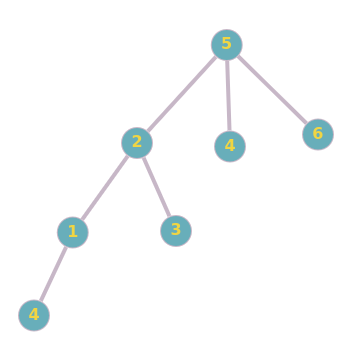
\includegraphics[width=0.2\textwidth]{figures2/arbol.png}
    \caption{Ejemplo de \'arbol}
\end{figure}

\textbf{Nota:} Cada una de las componentes conexas de un Bosque es un \'Arbol.

\textbf{Nota:} Un \'arbol es a la vez un bosque.

\begin{dfn}[\'Arbol Abarcador]
    Sea $G$ un grafo, se define $T$ como \'arbol abarcador de $G$ a un subgrafo en expansi\'on de $G$ que sea ac\'iclico y conexo.
\end{dfn}

\begin{teo}
    Todo grafo conexo tiene un \'arbol abarcador.
\end{teo}

\begin{dem}[V\'ia Constructiva]\end{dem}
Sea $G$ un grafo conexo, si es ac\'iclico, listo, $T = G$, si no, $G$ tiene ciclos, si se toma un ciclo de $G$ y se quita una arista esto no rompe la conexidad, y este proceso se puede realizar reiteradamente hasta que no queden m\'as ciclos, obteni\'endose as\'i un \'arbol abarcador de $G$.\\


\textbf{Nota:} N\'otese que el \'arbol abarcador no es \'unico para $G$, que adem\'as $|E(G)| \geq |E(T)|$ puesto que en el propio proceso de obtenci\'on de $T$ se quitan aristas de $G$ en cada paso y que para un grafo no conexo se puede obtener un \'arbol abarcador por cada componente conexa, gener\'andose as\'i un bosque.


\begin{figure}[H]
    \centering
    \begin{subfigure}[b]{0.8\textwidth}
    \centering
    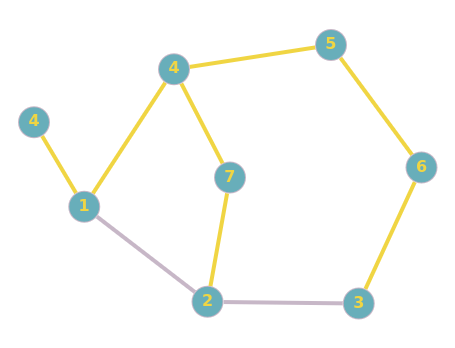
\includegraphics[width=0.30\textwidth]{figures2/arbolA1.png}
    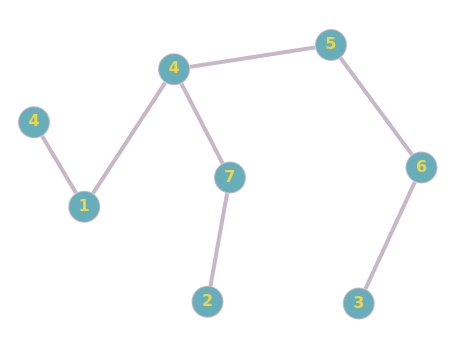
\includegraphics[width=0.30\textwidth]{figures2/T1.png}
    \caption{$G$ y posible $T$ \'arbol abarcador}
    \end{subfigure}
    \begin{subfigure}[b]{0.8\textwidth}
        \centering
    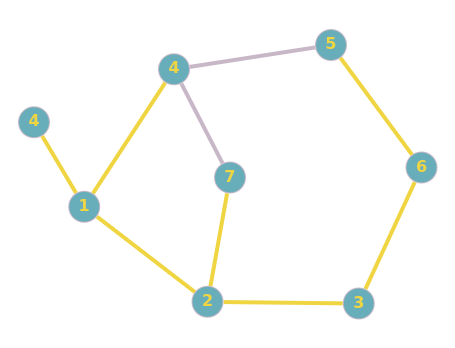
\includegraphics[width=0.30\textwidth]{figures2/arbolA2.png}
    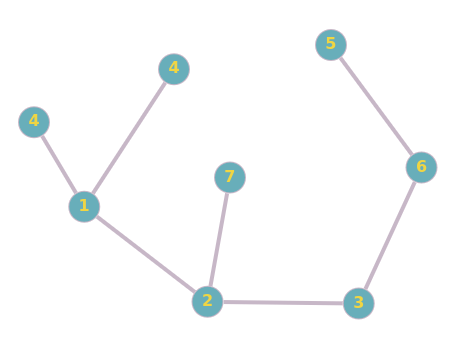
\includegraphics[width=0.30\textwidth]{figures2/T2.png}
    \caption{$G$ y otro posible $T$ \'arbol abarcador}
    \end{subfigure}
\end{figure} 

\begin{teo}[Teorema de las 6 equivalencias]
Sea $G$ tal que $n = |V(G)| \geq 2$, son equivalentes las siguientes proposiciones:

\begin{enumerate}
    \item $G$ es un \'arbol.
    \item $G$ no tiene ciclos y $|E(G)| = n-1$.
    \item $G$ es conexo y $|E(G)| = n-1$.
    \item $G$ es conexo pero si le quitas una arista deja de serlo.
    \item $G$ es ac\'iclico, pero si le agregas una arista se forma exactamente un ciclo.
    \item Todo par de v\'ertices en $G$ est\'an conectados exactamente por un camino simple. 
\end{enumerate}
\end{teo}

\begin{dem}[$P_1 \Rightarrow P_2 \Rightarrow P_3 \Rightarrow P_4 \Rightarrow P_5 \Rightarrow P_6 \Rightarrow P_1$]
    Para demostrar la equivalencia entre las proposiciones, la foma m\'as r\'apida es hacer un ciclo de implicaciones y demostrar cada una de ellas, as\'i para cualquier par de propiedades se puede demostrar que se llega de una a la otra a trav\'es de una cadena de transitividad.
\end{dem}
\begin{dem}[$P_1 \Rightarrow P_2$ V\'ia: Inducci\'on en $|V(G)| = n$] $G$ es un \'arbol $\Rightarrow$ $G$ no tiene ciclos y $|E(G)| = n-1$.\end{dem}

Caso base $n = 2$ Como $G$ es \'arbol, entonces es conexo, luego los dos v\'ertives tienen que estar unidos por una arista de donde $|E(G)| = 1 = n-1$.

Hip\'otesis $n$: Supongamos que para cualquier \'arbol de $n$ v\'ertices se cumple que este tiene $|E(V)| = n -1$.

Demostración $n+1$: Sea $G$ un grafo de $n+1$ v\'ertices, como por el teorema anteriormente demostrado sabemos que existen en $G$ al menos dos hojas, sea $v$ una hoja, $G' = G - v$ sigue siendo un \'arbol ya que quitar v\'ertices no produce ciclos y adem\'as como este v\'ertice tiene grado $1$ quitarlo no desconecta el grafo. Luego $G'$ es un \'arbol de $n$ v\'ertices, por lo que cumple con la hip\'otesis de inducci\'on y $|E(G')| = n-1$. Como $|E(G)| = |E(G')| +1$, ya que junto al v\'ertice $v$ se quita la arista que lo conectaba a $G$, entonces $|E(G)| = n-1+1 = n \blacksquare$.

\begin{dem}[$P_2 \Rightarrow P_3$ V\'ia: Directa] $G$ no tiene ciclos y $|E(G)| = n-1 \Rightarrow$ $G$ es conexo y $|E(G)| = n-1$. .\end{dem}

Sean $Cc_1, Cc_2..., Cc_k$ las componentes conexas de $G$, con $n_1, n_2,.., n_k$ v\'ertices cada una,  como $G$ es ac\'iclico, entonces cada una de sus componentes conexas es un \'arbol luego 

$$ |E(G)| = \sum_{i = 1}^{k} |E(Cc_i)| = \sum_{i =1}^{k} (n_i -1) = \sum_{i =1}^{k} n_i -k = n -k$$

Luego $k = 1$ siendo $G$ conexo $\blacksquare$.

\begin{dem}[$P_3 \Rightarrow P_4$ V\'ia: \'Arbol Abarcador] $G$ conexo y $|E(G)| = n-1 \Rightarrow$ $G$ es conexo pero si se le quita una arista se desconecta.\end{dem}

Esto es equivalente a demostrar que para que un grafo sea conexo tiene que tener una cantidad de aristas mayor o igual a $n-1$. Ya que si esto se cumple, al $G$ ser conexo y tener $n-1$ aristas si le quitamos una perder\'ia su conexidad.

Sea $G$ conexo, entonces se puede obtener $T$ \'arbol abarcador de $G$, donde $|E(G)| \geq |E(T)| = n-1$ luego si $G$ conexo $|E(G)| \geq n-1 \blacksquare$. 


\begin{dfn}
    Sea $G$ un grafo, la secuencia de grados de $G$ es una lista con los grados de los v\'ertices de $G$. Un grafo con secuencia $d$ se dice que \textbf{realiza} $d$.
\end{dfn}

\begin{dfn}[Secuencia gr\'afica]
    Una secuencia $d_1, d_2, ..., d_n$ se dice gr\'afica si hay un grafo que la realiza.
\end{dfn}

\begin{teo}
    Una secuencia de $n$ n\'umeros no negativos $d_1, d_2,..., d_n$ es la secuencia de grados de un pseudografo $\Leftrightarrow \sum_{i=1}^{n} d_i$ es par.
\end{teo}

\begin{dem}[$\Rightarrow$] Si $d_1, d_2,..., d_n$ es la secuencia de grados de un pseudografo  $\Rightarrow \sum_{i=1}^{n} d_i$ es par\end{dem}

La demostraci\'on es an\'aloga a la de la suma de los grados de un grafo es el doble del n\'umero de aristas, lo que en este caso se admiten aritsas m\'ultiples que de igual modo incrementan en $1$ el grado de cada v\'ertice en el que inciden y lazos que incrementan en $2$ el grado del v\'ertice en el que inciden.

\begin{dem}[$\Leftarrow$]  $\sum_{i=1}^{n} d_i$ es par $\Rightarrow$ $d_1, d_2,..., d_n$ es la secuencia de grados de un pseudografo \end{dem}

Para demostrarlo basta con construir un pseudografo con $n$ v\'ertices tal que los grados de estos coincidan con la secuencia. Para ello, creamos $n$ v\'ertices y para aquellos $d_i$ que sean pares, al v\'ertice $i$ le ponemos $\frac{d_i}{2}$ lazos, y para los $d_i$ que son impares al v\'ertice $i$ le ponemos $\frac{d_i -1}{2}$ lazos, como $\sum_{i=1}^n d_i$ es par, entonces hay una cantidad par de v\'ertices con grado impar, a cada uno le falta agregarle una arista m\'as para que su grado coincida con su $d_i$ asignado, por lo que se unen en parejas mediante una arista.

\end{document} 